\section{Operating System Considerations}
\label{os-considerations}
%\subsection{Evolved Embedded Applications}

In the first evolutionary cycle of embedded devices, applications were written
as an integral part of the runtime environment on the device. The second
cycle brought operating systems like TinyOS, Contiki, FreeRTOS and conceptually
separated application and OS code. The development became easier allowing
complexity of applications to remain manageable as they grew. However, the resulting
code was still compiled to a monolithic image and uploaded to the device.

Now the third evolutionary cycle is emerging: multiple and independently
developed application have to co-exist on the same device (like in Pebble watch);
and embedded devices are becoming modular. The latter is evident with
multi-billion companies like Samsung, Telefonica and GE innovating with SimBand, Wzzard, ThinkingThings, Spotter UNIQ.
%~\endnote{http://www.samsung.com/us/globalinnovation/innovation_areas/}, Wzzard
%~\endnote{http://bb-smartsensing.com/wzzard-sensing-platform/}, ThinkingThings
%~\endnote{http://www.thinkingthings.telefonica.com/}, Spotter UNIQ
%~\endnote{https://www.quirky.com/shop/982-spotter-uniq-customizable-multipurpose-sensor}
The aim is to create a core hardware platform where adding sensory
peripherals is done by the consumer in a Lego-like fashion while the developer compiles the
application with the provided SDK. %this paragraph needs rephrasing

These trends completely change the way applications for the embedded devices
have been developed over the last five decades. Developers have very little control over the
application execution model, its coexistence with other application, and which
peripherals are connected to the embedded device. Instead application developers
expect that the underlying operating system will perform fair resource allocation,
protecting the application from malicious or malfunctioning applications and
peripherals. 

Given the paradigm shift in embedded devices we propose a design for a new operating system,
\name, that supports a combinations of goals:


\begin{itemize}
  \item Event-driven execution model
  \item Loadable applications, services and drivers
  \item Robust, Reliable and Safe %isolation
  \item Energy Efficient 
\end{itemize}



\subsection{Application execution model}
\begin{figure}
 \centering
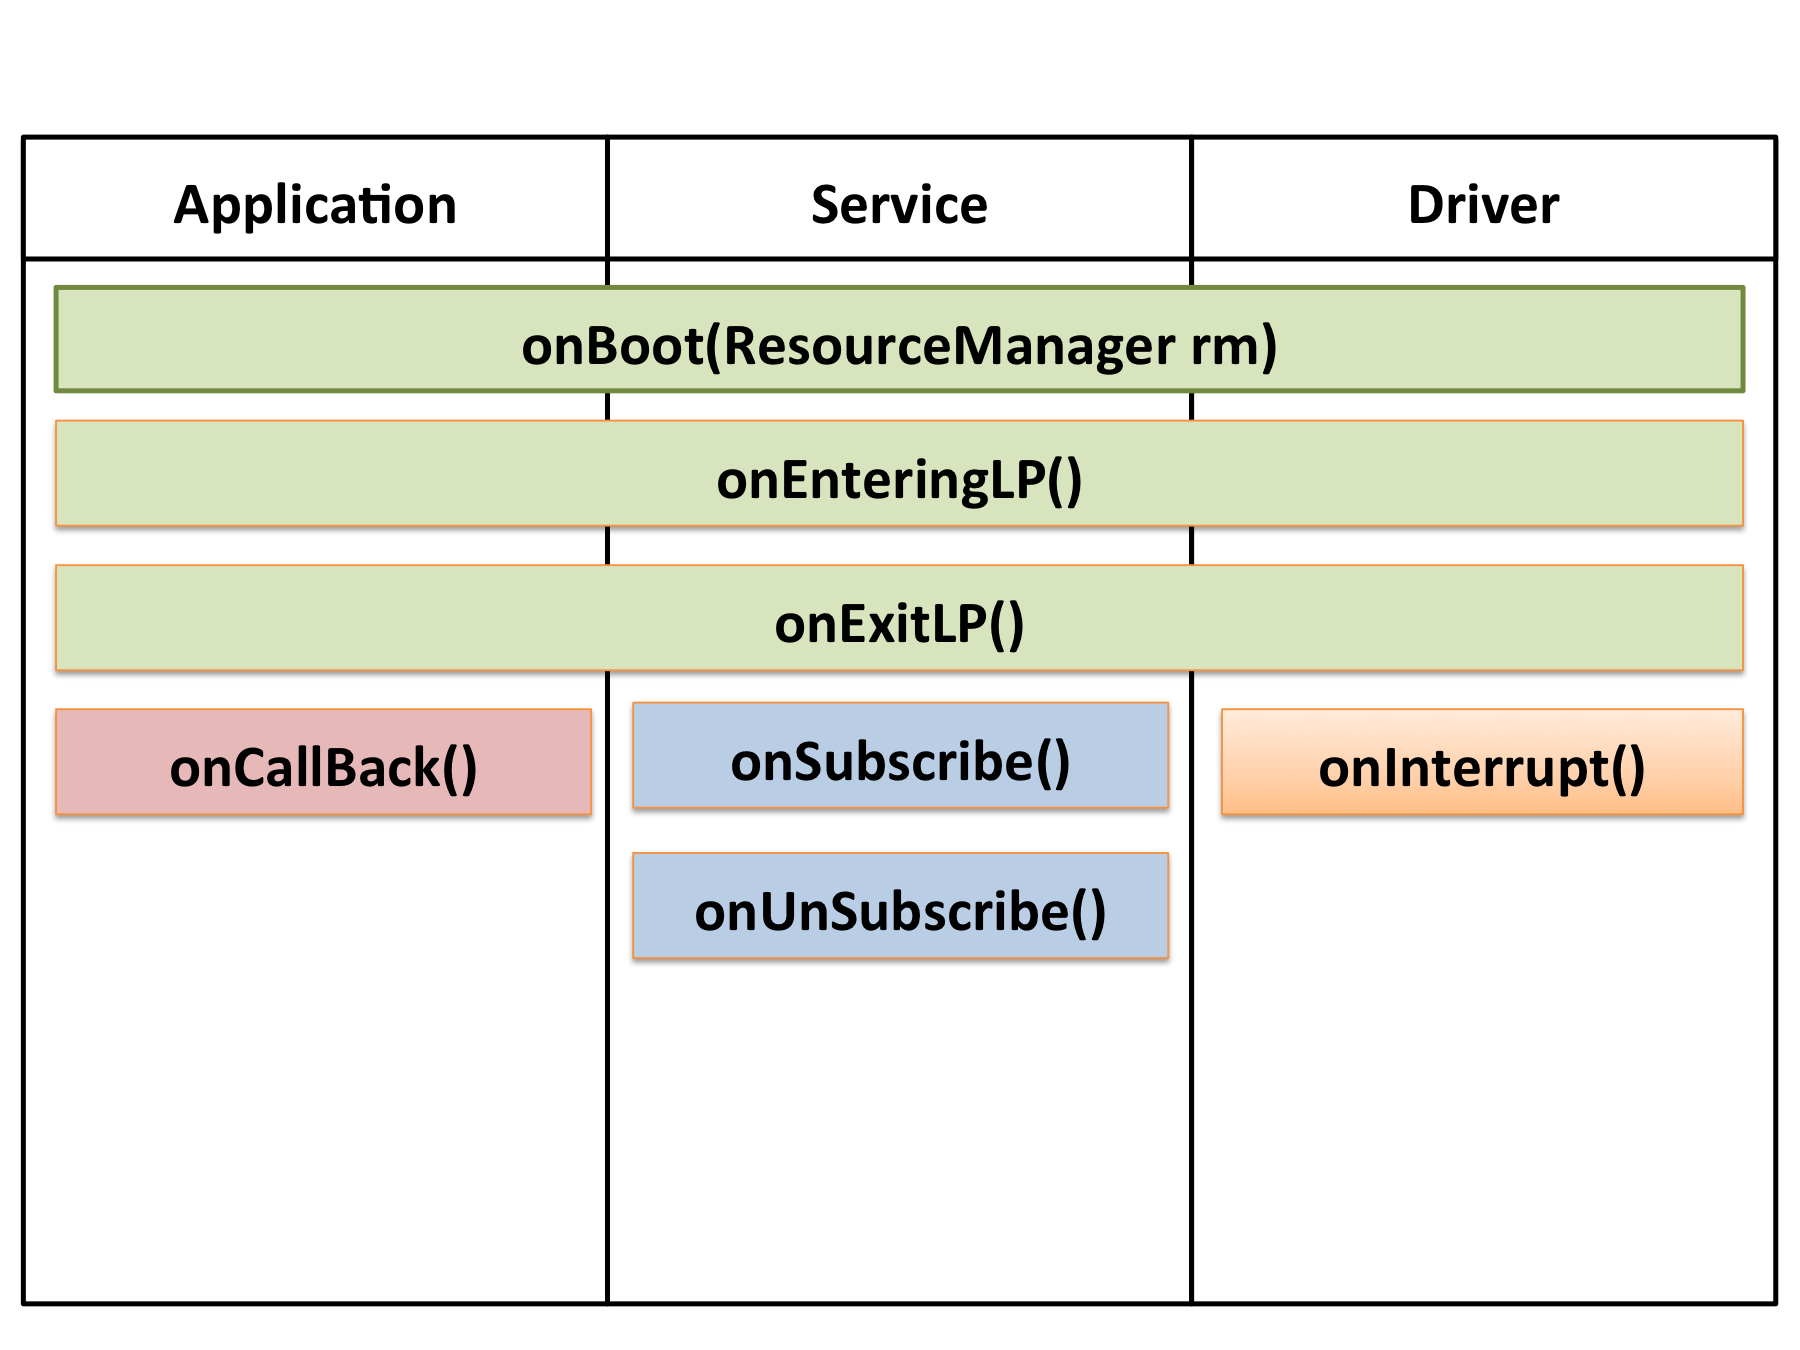
\includegraphics[width=1\columnwidth]{img/appcycle.png}
\caption{Runnable life cycle.}
 \label{fig:appcycle}
\end{figure}


\subsection{Loadable applications, services and drivers}
% should we talk about what tock does or jsut focut on the new generations of
% os instead? I prefere the considerations so there is no overlapp and
% inconsistencies in text

\name provides a system-call interface. This
allows developers to write applications in any language that can support the
ABI. For example, the \name kernel is written in Rust~\cite{rust}, applications
can be trivially written in C, and we have completed a port of Lua~\cite{lua}.

\subsection{Robust, Reliable and Safe}
%to be rewriten
 \name follows previous operating systems in separating
drivers for core peripherals (SPI, USART, GPIO, etc) and device drivers (radio,
flash, etc) into separate layers. \name differs from previous operating systems
in enforcing safety policies on device drivers through the Rust type system.
\name prevents drivers from subverting Rust's memory safety by restricting
device drivers to a safe subset of the Rust language.~\endnote{Rust allows code
to circumvent the type system using the \tt{unsafe} keyword. \name uses a
compiler flag that disallows this keyword when compiling device drivers.} \name
also ensures, at compile time, that at most one driver has access to a specific
hardware resource---multiplexing must be done explicitly in the core peripheral
driver or through an intermediate interface. Finally, \name ensures device
drivers cannot corrupt kernel memory through careful choice of interfaces. \name
ensures that \name does not protect the kernel from denial of service attacks by
drivers. %wait what does this last sentence mean?

{\bf Reliability}. Unlike most desktop and server applications, embedded
applications must continue to run without end-user intervention. There is no
console to indicate to the user that an application has crashed. Even if a crash
could be communicated to the user, there is little action they could take. While
a Blue-Screen-Of-Death is annoying on a desktop or server, it is unacceptable in
embedded systems. Unlike other embedded operating systems, \name does not allow
applications to corrupt the kernel or other applications. Moreover, certain
parts of the kernel (e.g. contributed device drivers) are isolated using
a strong language type system.

\subsection{Energy Efficient}


\subsection{Scheduling}
% this is important part but how much place we have to talk about it.

